\documentclass[12pt]{article} \usepackage{COSC420style} \usepackage{soul}
\usepackage{booktabs}
\usepackage{verbatim}
\usepackage{hyperref}
\usepackage{graphicx}
\usepackage{subcaption}
\papercode{COSC420}

\title{Transformer based language model}

\author{Jake \textsc{Norton}} \studentid{5695756}

\reportdate{\today}

\begin{document}

\maketitle

\section{Introduction}

This report discusses the development and evaluation of a text generation framework using the novels
\textit{Pride and Prejudice} and \textit{War and Peace}.  Many of the decisions made here were close
to arbitrary in nature due to time constraints, and I did not get to explore as much as I would have
liked. However, I do believe that the models created are still adequate at creating text that is at
least interesting. In terms of text choice, I decided to use all of both books. This provided the
most data, but at a cost of potential bias. This was a trade off I was willing to take as I hoped
that generally the model would perform better, if skewed towards talking \textit{War and Peace}.
\section{Task 1: Tok2Vec Encoder}

\subsection{Methodology}

Word2vec embeddings can be created using two primary approaches: Skip-gram (SG) and Continuous Bag
of Words (CBOW). These methods are essentially opposites; CBOW predicts a word based on the context
of surrounding words, while Skip-gram, conversely, predicts the surrounding context from a given
word. CBOW is effective for identifying common links among frequently used words, making it ideal
for smaller datasets where the focus is on simpler relationships that require less data to discern.
However, the method's tendency to average context can lead to a less detailed understanding. In
contrast, Skip-gram excels in capturing more complex relationships but requires more data and longer
training times. Each position in the context window must be trained separately, unlike CBOW, which
integrates all context simultaneously.

I chose to use Skip-gram for its potential to uncover interesting patterns despite the limitations
of our dataset. The exploration process was somewhat limited due to early corruption in my
token-to-vector models. To expedite the process, I saved the encoded vectors of the entire corpus to
be read in each time, which significantly reduced processing time. However, at some point, the
dataset I believe the saved encoded dataset was corrupted, as the predictions were always the tokens \textit{i},
\textit{\ae}, \textit{=}. Unfortunately the t-SNE plots of the models indicated that they
were generally successful in clustering semantically similar words and so I didnt not realise the
models were corrupted until after I began training the transformer models. After reencoding the
dataset this pattern went away on all versions of the model.

\begin{table}[htbp]
	\centering
	\caption{Frequency of Words with Different Context Window Sizes}
	\label{tab:word_frequencies}
	\begin{tabular}{cccccc}
		\toprule
		\multicolumn{2}{c}{Context window size 3} & \multicolumn{2}{c}{Context window size 4} & \multicolumn{2}{c}{Context window size 5}                                                \\
		\cmidrule(r){1-2} \cmidrule(lr){3-4} \cmidrule(l){5-6}
		Token                                     & Probability                               & Token                                     & Probability & Token            & Probability \\
		\midrule
		\textbackslash s                          & 0.0655                                    & \textbackslash s                          & 0.0673      & \textbackslash s & 0.0911      \\
		the                                       & 0.0322                                    & ,                                         & 0.0329      & the              & 0.0446      \\
		,                                         & 0.0301                                    & the                                       & 0.0315      & ,                & 0.0419      \\
		and                                       & 0.0205                                    & and                                       & 0.0216      & .                & 0.0272      \\
		.                                         & 0.0185                                    & .                                         & 0.0210      & and              & 0.0260      \\
		of                                        & 0.0176                                    & of                                        & 0.0210      & of               & 0.0238      \\
		to                                        & 0.0169                                    & to                                        & 0.0150      & to               & 0.0175      \\
		a                                         & 0.0114                                    & in                                        & 0.0112      & a                & 0.0135      \\
		in                                        & 0.0100                                    & a                                         & 0.0107      & in               & 0.0121      \\
		his                                       & 0.0086                                    & his                                       & 0.0084      & his              & 0.0097      \\
		was                                       & 0.0076                                    & was                                       & 0.0075      & was              & 0.0083      \\
		that                                      & 0.0073                                    & with                                      & 0.0070      & with             & 0.0076      \\
		he                                        & 0.0067                                    & that                                      & 0.0063      & that             & 0.0071      \\
		her                                       & 0.0064                                    & he                                        & 0.0061      & he               & 0.0069      \\
		with                                      & 0.0064                                    & had                                       & 0.0053      & her              & 0.0063      \\
		'                                         & 0.0061                                    & at                                        & 0.0053      & had              & 0.0059      \\
		had                                       & 0.0052                                    & on                                        & 0.0051      & at               & 0.0056      \\
		at                                        & 0.0050                                    & her                                       & 0.0051      & '                & 0.0054      \\
		it                                        & 0.0046                                    & '                                         & 0.0049      & on               & 0.0052      \\
		"                                         & 0.0045                                    & for                                       & 0.0041      & "                & 0.0051      \\
		\bottomrule
	\end{tabular}
\end{table}

Regarding the context window for the model, I found that a size below 3 yielded poor results in
prediction tests. I experimented with sizes up to 5, but choosing between 3, 4, and 5 proved
challenging. The larger the context window, the more it prioritized punctuation, as shown in
Table~\ref{tab:word_frequencies}. Eventually, I opted for a context window of 4, aiming to balance
the difference and reduce training time. I was ultimately satisfied with the punctuation versus text
balance, though the model still occasionally struggles with quotations. Models with a context window
of 4 generally showed a nicely distributed clustering of semantically similar words such as "would,
should, could, must, shall."

To determine the vocabulary size, I performed a rough count of unique words using a series of Bash
commands\footnote{bash command: \texttt{tr '[:upper:]' '[:lower:]' < combined\_books\_text | tr -d
'[:punct:]' | tr ' ' '\textbackslash{}n' | sort | uniq | wc -l}}, resulting in approximately 25,000
words. However, this count included many duplicates or near-duplicates due to punctuation, as
demonstrated by the list of variations of the word 'your'.

\begin{itemize}
	\item   ‘your
	\item   “your
	\item   your
	\item   “you’re
	\item   you’re
\end{itemize}

To maximize coverage while managing
memory and model size limitations, I capped the token count at 5,000, reasoning that if ChatGPT
operates effectively with around 50,000 unique tokens, 10\% should be sufficient for a corpus of this
size.

To find out the vocab size I calculated a rough count of unique words over the whole corpus which gave me approximately 25,000
words. From the eye test, though, there were many duplicates/close duplicates in there, mainly due
to punctuation, for example.


To capture as much as I could I went up to 5000 tokens which was the limit due to memory and model
size concerns at higher token counts. Additionally, if chatgpt can manage with only ~50000 unique
tokens, 10\% for a corpus of this size seems reasonable to me.

I also explored various sizes for the hidden layer dimensions, ranging from 32 to 512. Limited
testing made it difficult to determine the best size quantitatively, though it was evident that
dimensions of 32 and 64 were insufficient, as they resulted in a noticeable skew in the graphical
outputs. While t-SNE reduces dimensionality and may not make a linear skew inherently problematic,
my interpretation was that such skewness indicated a simpler embedding representation.

\begin{itemize}
	\item \textbf{Context Window}: 4
	\item \textbf{Hidden Layer Dimension}: 256
	\item \textbf{Vocab Size}: 5000
\end{itemize}

\begin{figure}[htbp]
	\centering
	\begin{subfigure}[b]{0.45\textwidth}
		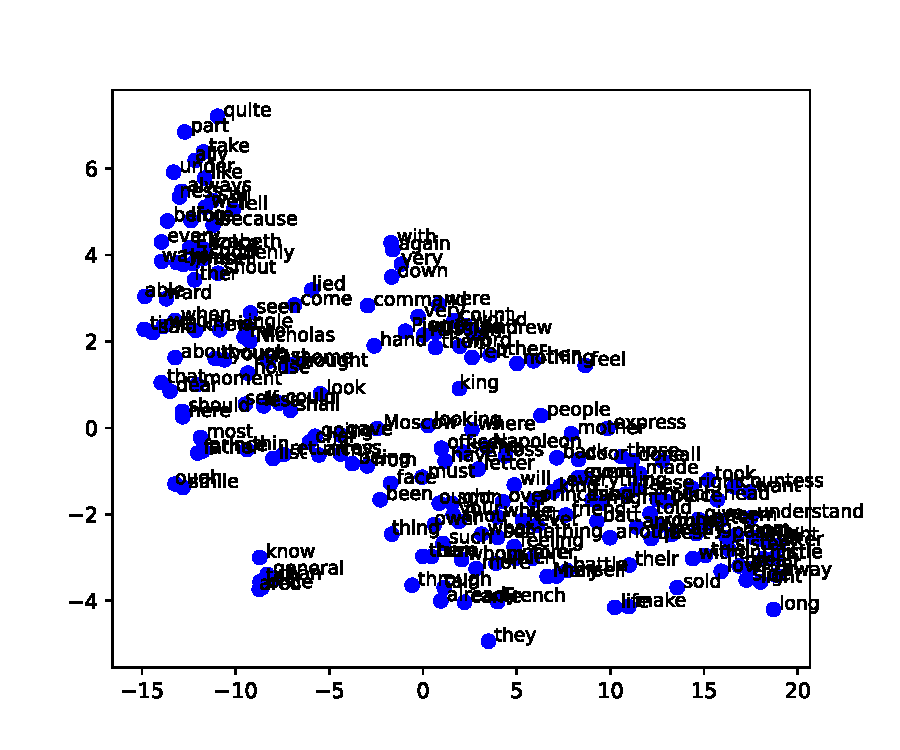
\includegraphics[width=\textwidth]{./figures/dim_32_ctx_1_embedding.pdf}
		\caption{neurons: 32, context window of 1}
		\label{fig:32_1}
	\end{subfigure}
	\begin{subfigure}[b]{0.45\textwidth}
		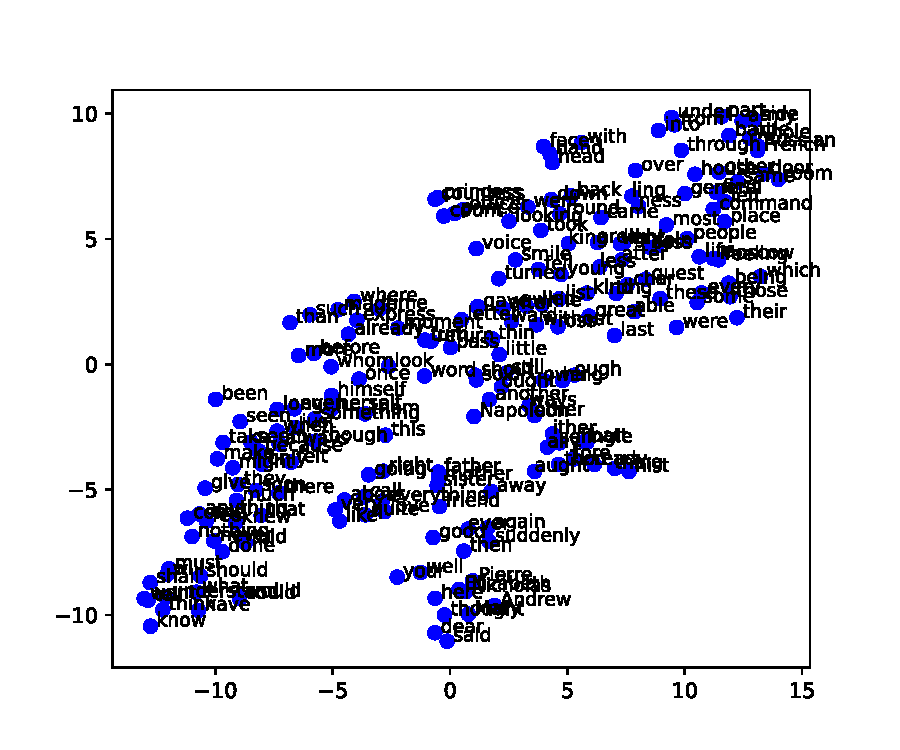
\includegraphics[width=\textwidth]{./figures/dim_32_ctx_4_embedding.pdf}
		\caption{neurons: 32, context window of 4}
		\label{fig:32_4}
	\end{subfigure}
	\newline % starts a new line
	\begin{subfigure}[b]{0.45\textwidth}
		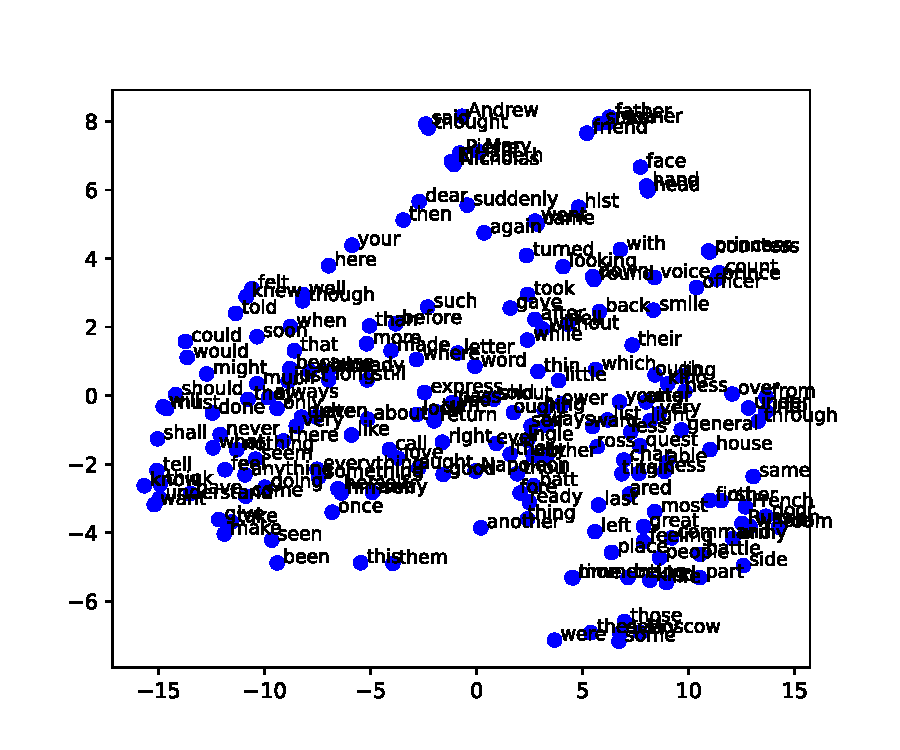
\includegraphics[width=\textwidth]{./figures/dim_64_ctx_3_embedding.pdf}
		\caption{neurons: 64, context window of 3}
		\label{fig:64_3}
	\end{subfigure}
	\begin{subfigure}[b]{0.45\textwidth}
		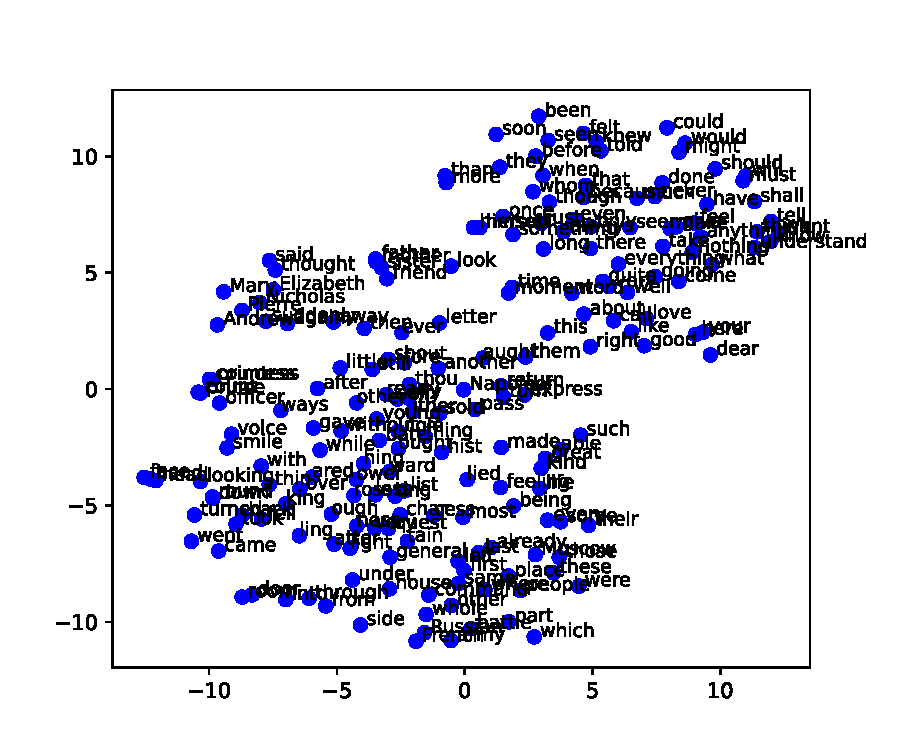
\includegraphics[width=\textwidth]{./figures/dim_64_ctx_5_embedding.pdf}
		\caption{neurons: 64, context window of 5}
		\label{fig:64_5}
	\end{subfigure}
	\caption{t-SNE plots of embedding space with varying sizes of neurons and context
		windows}
	\label{fig:small_embeddings}
\end{figure}

\begin{figure}[htbp]
	\centering
	\begin{subfigure}[b]{0.45\textwidth}
		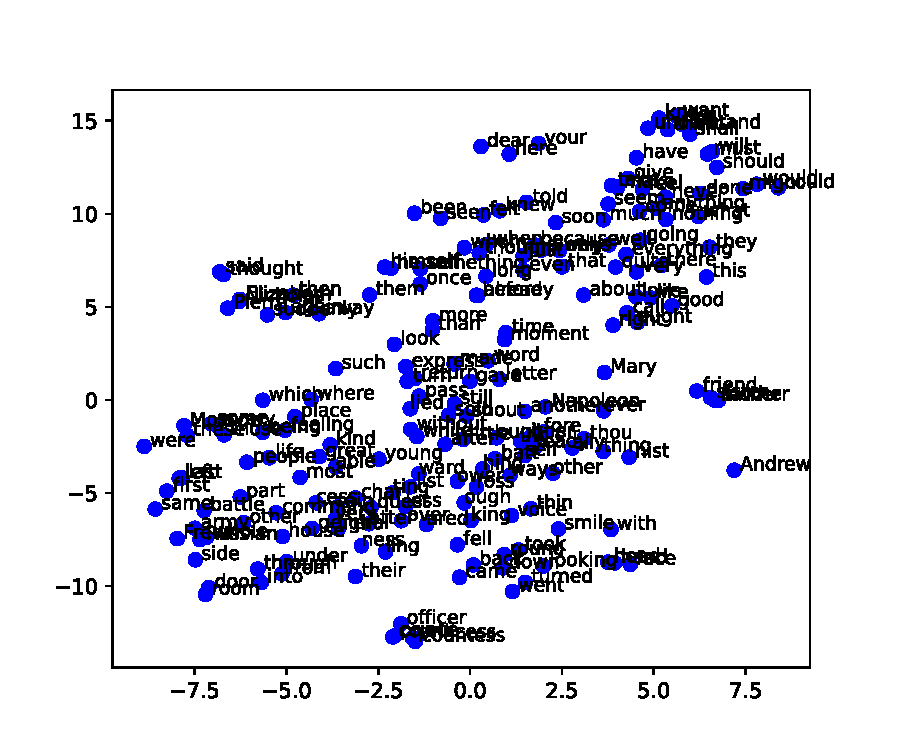
\includegraphics[width=\textwidth]{./figures/dim_64_ctx_4_embedding.pdf}
		\caption{neurons: 64, context window: 4}
		\label{fig:64_4}
	\end{subfigure}
	\hfill % Add horizontal space between the first and second subfigures on the same row
	\begin{subfigure}[b]{0.45\textwidth}
		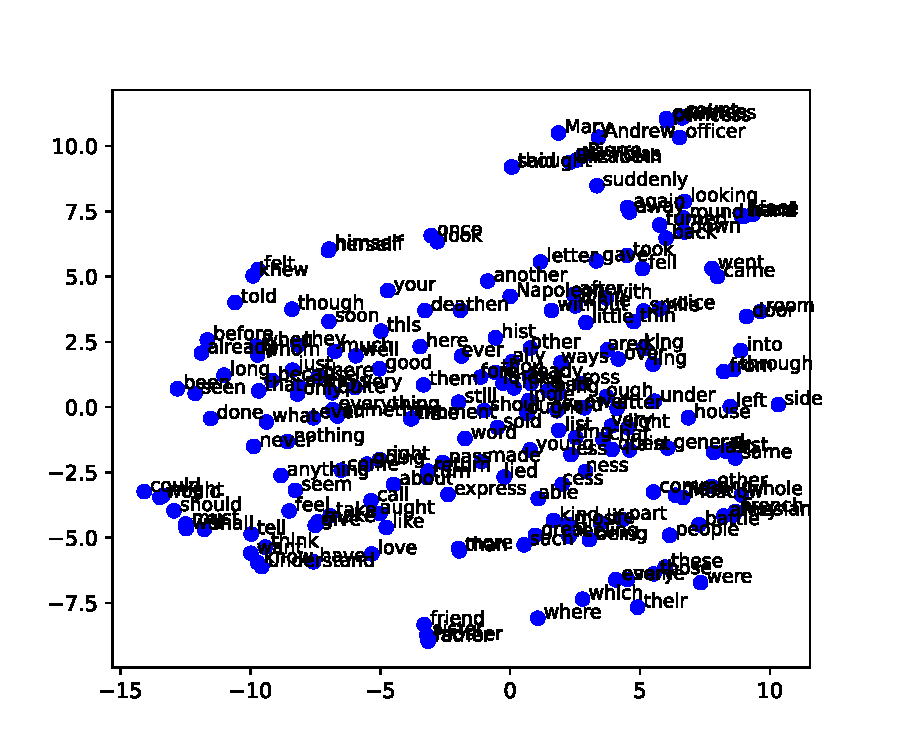
\includegraphics[width=\textwidth]{./figures/dim_128_ctx_4_embedding.pdf}
		\caption{neurons: 128, context window: 4}
		\label{fig:128_4}
	\end{subfigure}
	\newline % Starts a new line for the next row: subfigures
	\begin{subfigure}[b]{0.45\textwidth}
		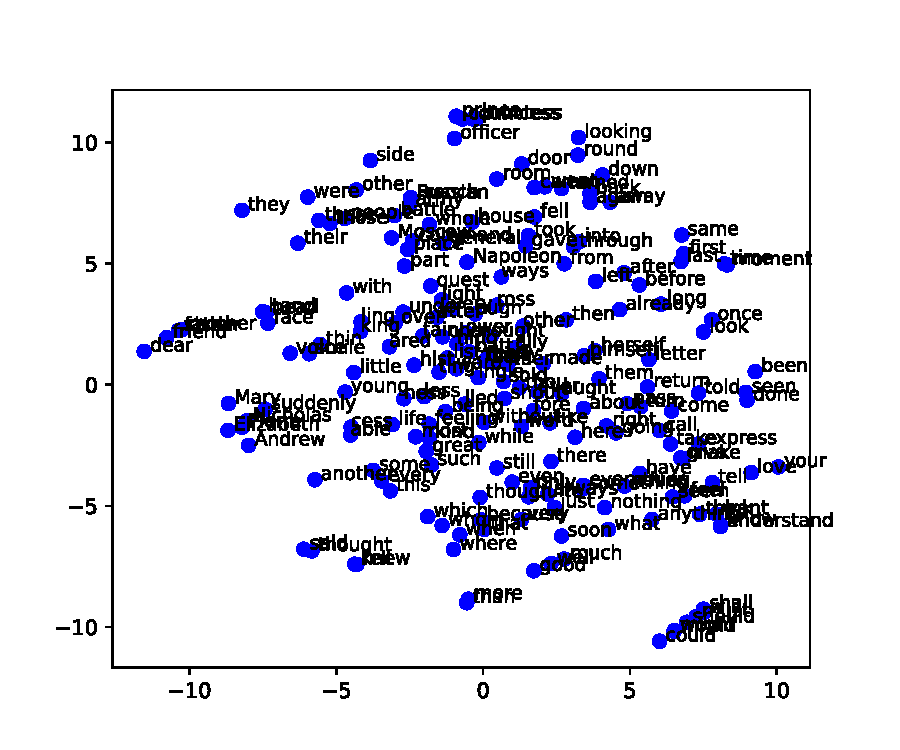
\includegraphics[width=\textwidth]{./figures/dim_256_ctx_4_embedding.pdf}
		\caption{neurons: 256, context window: 4}
		\label{fig:256_4}
	\end{subfigure}
	\hfill % Add horizontal space between the first and second subfigures on the same row
	\begin{subfigure}[b]{0.45\textwidth}
		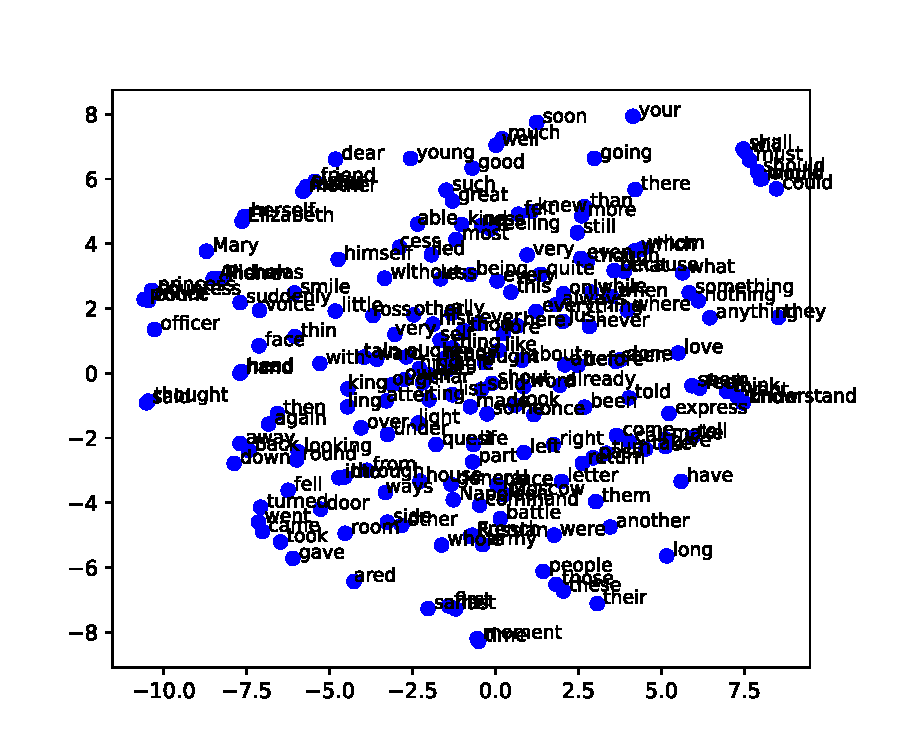
\includegraphics[width=\textwidth]{./figures/dim_512_ctx_4_embedding.pdf}
		\caption{neurons: 512, context window: 4}
		\label{fig:512_4}
	\end{subfigure}
	\caption{t-SNE plots of embedding space with varying sizes of neurons and context windows}
	\label{fig:larger_embeddings}
\end{figure}


\section{Task 2: Transformer-based Text Prediction}

\subsection{Methodology}

Using the transformer provided, I adjusted the model to take my 256 dimension embeddings, as well to
be able to use one-hot vectors as input. I chose to only train for 1 epoch, partly due to time
constraints, and due to the validation accuracy not improving over multiple epochs.  After finding
this, I did not both including the validation split and went by qualitative measures to ascertain
the performance.
\subsection{Implementation}

The models were all trained on all of the training data, this has influenced it to prefer to talk
more about things seen in War and Peace, though sections of Pride and Prejudice still show through.

\begin{table}[htbp]
	\centering
	\caption{Performance Metrics for Different Configurations}
	\label{tab:performance_metrics}
	\begin{tabular}{cccccc}
		\toprule
		\multicolumn{6}{c}{Transformer with Embeddings}                                                                  \\
		\midrule
		\textbf{Attention Heads} & \textbf{Transformer Layers} & \textbf{DFF} & \textbf{Loss} & \textbf{Masked Accuracy} \\
		4                        & 4                           & 256          & 2.8427        & 0.4136                   \\
		4                        & 4                           & 512          & 2.6718        & 0.4373                   \\
		4                        & 6                           & 256          & 2.6647        & 0.4402                   \\
		4                        & 6                           & 512          & 2.4718        & 0.4695                   \\
		16                       & 4                           & 256          & 2.3300        & 0.4995                   \\
		16                       & 4                           & 512          & 2.2095        & 0.5197                   \\
		16                       & 6                           & 256          & 2.0522        & 0.5551                   \\
		16                       & 6                           & 512          & 1.9590        & 0.5725                   \\
		\midrule
		\multicolumn{6}{c}{Transformer using One-hot Representation}                                                     \\
		\midrule
		4                        & 4                           & 256          & 2.2441        & 0.5154                   \\
		4                        & 4                           & 512          & 2.1719        & 0.5289                   \\
		4                        & 6                           & 256          & 2.0241        & 0.5586                   \\
		4                        & 6                           & 512          & 1.9068        & 0.5823                   \\
		16                       & 4                           & 256          & 1.6985        & 0.6311                   \\
		16                       & 4                           & 512          & 1.6726        & 0.6358                   \\
		16                       & 6                           & 256          & 1.4977        & 0.6802                   \\
		16                       & 6                           & 512          & 1.4662        & 0.6856                   \\
		\bottomrule
	\end{tabular}
\end{table}


\subsection{Results}

Analysis of training and, if applicable, validation accuracies. Qualitative assessment of the text
generation capabilities for both the one-hot encoded and Tok2Vec encoded models. Comparison of
outputs when prompted with extracts from the training texts versus new, unseen prompts.

\section{Task 3: Report and Evaluation}

\subsection{Overview of Tasks}

Summary of the methodologies and key decisions taken during the project.

\subsection{Evaluation and Comparison}

Critical evaluation of the models based on the tasks' results, discussing the effectiveness and
limitations of each approach.

\section{Conclusion}

Reflections on the project outcomes, lessons learned, and potential areas for future research.

\section{References}
% Use BibTeX or a manually curated bibliography.

\end{document}
